\documentclass[twocolumn]{scrartcl}
\usepackage[cm]{fullpage}
\usepackage{hyperref}
\usepackage{graphicx}
\usepackage[backend=biber]{biblatex}
\addbibresource{report.bib}

\title{Classification of Wine Quality}
% Do NOT write your names here!
\author{Anonymous Authors}
\begin{document}
\maketitle

\section{Introduction}

The following report outlines our attempts to use common classification
algorithms to predict the wine quality depending on the given features.
We use a data set from the UCI Machine Learning Repository
\footnote{\url{http://archive.ics.uci.edu/ml/datasets/Wine+Quality}} \parencite{data}.

\subsection{Data Description}

The data set contains of 4898 data points, each of them described by 11 features
and an integer quality label ranging from 3 to 9.
Note that the distribution of the quality is unbalanced:
More than 90\% of the data points are assigned to a quality between 5 and 7 (Figure \ref{fig:unbal}).

\begin{figure}[h]
    \centering
    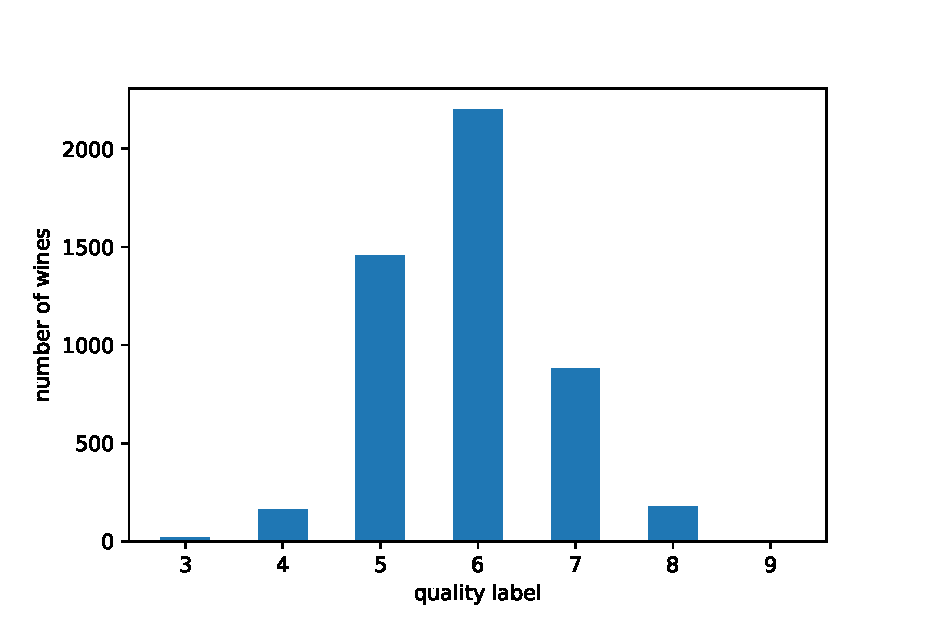
\includegraphics[width=\linewidth]{images/unbalanced.eps}
    \caption{distribution of quality}
    \label{fig:unbal}
\end{figure}

\subsection{Data preprocessing}

To simplify our problem we assigned new class labels 0, 1 and 2. We assign class 0 (bad) to wines ranging in qualities 3-5,
class 1 (medium) to wines labeled with quality 6 and class 2 (good) to wines with quality greater than 6.
We further decided to use classification instead of regression.
Though, it should be noted that we also examine algorithms (e.g. ridge classifier) that use regression to classify the data points
and using regression should therefore yield similar results in our case.
This doesn't come as a surprise, considering that the classes can obviously be linearly ordered.

\subsection{Cross-Validating the data}
The goal of cross validation is to achieve the accuracy of out-of-training data with using only the training data itself. So we don't have to separate the data into two different groups, instead we train the model on all of the data set.

In out project we use the cross\_val\_score helper function to calculate the mean and the accuracy\footnote{\url{https://scikit-learn.org/stable/modules/cross_validation.html\#computing-cross-validated-metrics}} of the different models.

%not yet decided which to use
\section{Ridge Classification}
\subsection{Description}
Ridge Classifier implements Ridge regression.
Ridge regression (one of it's many names) is a linear regularization method
\footnote{\url{https://en.wikipedia.org/wiki/Tikhonov_regularization}}
that addresses some of the Ordinary Least Squares problems
\footnote{\url{https://scikit-learn.org/stable/modules/linear_model.html\#ridge-regression}}
in which if there is no unique answer the estimator will lead to over fitting or under fitting and the result will not be as accurate as by using other methods.

In our project we have implemented the RidgeClassifier function from the Scikit-learn library.
\subsection{Cross-Validation}
We used the RandomizedSearchCV function from the Scikit-learn library to perform cross-validation on different combinations of hyperparameters. In this case we tried out settings for normalization and different values for the regularizition parameter alpha. The following combination returned the best results for us:

\begin{itemize}
    \item{fit intercept: True}
    \item{normalize: False}
    \item{alpha: 0.0017}
    \item{test score mean: 0.56}
    \item{accuracy: 0.56 (+/- 0.08)}
\end{itemize}

\section{Multi Layer Perceptron}
\subsection{Description}
Multi Layer Perceptron (MLP) is a supervised learning algorithm and is a function approximator that can be used for classification and regression which is widely used in neural network algorithms \footnote{\url{https://machinelearningmastery.com/neural-networks-crash-course/}}.
In this structure, a single neuron is represented by a single perceptron and when considering many of them, they represent the entire neural network. In this method, multiple layers (two or more with one or more additional hidden layers) and non-linear methods are used.One layer is simply one row of neurons. A simple MLP with only one hidden layer is represented in Figure \ref{fig:mlp} (Figure credit \footnote{\url{http://neuroph.sourceforge.net/tutorials/MultiLayerPerceptron.html}}).

\begin{figure}[h]
    \centering
    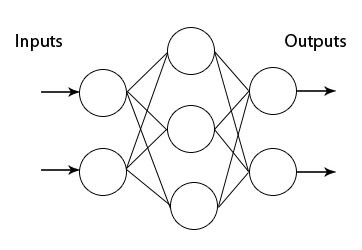
\includegraphics[width=\linewidth]{images/mlp.jpeg}
    \caption{Simple MLP with one hidden layer}
    \label{fig:mlp}
\end{figure}

We have used the MLPClassifier function (rather than MLPRegressor although both could be used on our chosen data set) from Scikit-learn's Neural Network library.

\subsection{Cross-Validation}
We again perform cross-validation on combinations of hyperparameters: These included different activation functions (logistic, tanh, relu, identity), regularizations, learning rates and hidden layer sizes. Because RandomizedSearchCV is not exhaustive the results are slightly different each run. A good choice of hyperparameters would be:
\begin{itemize}
    \item{activation: logistic}
    \item{alpha: 0.05}
    \item{hidden layer sizes: (100,)}
    \item{initial learning rate: 0.0005}
    \item{test score mean: 0.54}
\end{itemize}
It should be noted that in the case of MLPs every run returns a different classifer, even with the same hyperparameters so apart from the choice of the activation function other combinations of hyperparameters could yield similar results.

\section{Random Forest Classification}
\subsection{Description}
Random Forest is also a supervised learning algorithm that is widely used for solving classification and regression problems. The idea behind this method is to increase the classification accuracy (a.k.a aim for lower variance) by using bootstrap aggregating (or bagging) algorithms. Generally speaking, the gross idea behind Random Forest Classification is to use the bagging method to split up a decision tree into two different trees. When one does that enough times, there is a large amount of trees (hence the name- "forest) which gives the possibility to gather more information for analysis and therefore better accuracy. \footnote{\url{https://towardsdatascience.com/the-random-forest-algorithm-d457d499ffcd}}.

In this project we used the RandomForestClassifier algorithm from the Scikit-learn library.
\subsection{Results}
Varying the number of trees we get a test score mean of 0.58 and an accuracy of 0.58 (+/- 0.03) for using 659 trees.

\section{Gaussian Process Classification}
\subsection{Description}
Gaussian Processes algorithms could be also used for both classification and regression problems. A Gaussian process is a stochastic process with a Gaussian normal distribution kernel. This type of algorithm takes all the points that are available and measures the similarity between them to predict a value for a value for a future point.
The principle behind this classification method is the assumption that the tested data is normally distributed so this method should, in theory, work poorly on data that is not distributed in such a matter. In practice it could be observed that Gaussian processes work rather good on most data and the performance is not so accurate when the data set contain more than a dozen or a couple dozen of features.
\footnote{\url{https://www.kaggle.com/residentmario/gaussian-process-regression-and-classification}}.
Luckily, our wine quality data set has only 11 features, which should reproduce satisfactory results.

To implement the Gaussian Process Classification algorithm, we used the GaussianProcessClassifier method from the Scikit-learn library.

\subsection{Results}

Without cross-validation we get a score of 0.45.

\section{Comparison}

The Random Forest Classifier seems to work best when comparing the scores. The most efficient algorithm for us was Ridge Classification which takes a very short amount of time compared to other models and returns scores which are among the better ones.

\section{Conclusion}
With different models trying to classify the data the results remain mediocre at best. While some algorithms perform better than others, the scores are quite similar across all chosen models. As it gets more difficult to separate the classes more data is needed to take it to the next level, especially for MLPs. Another approach would be a thorough statistical analysis to understand which additional preparation steps could be beneficial. For example, every time we performed cross-validation the default metrics of the models have been used respectively. If the dataset is better understood, different, possibly more suitable metrics could be considered. As a conclusion we discovered that data preprocessing and preparation is much more important than we initially assumed. With dozens of algorithms it becomes difficult to get a grasp on which to use in different scenarios.

\printbibliography


\end{document}
